%%----------------------------------------------------------------------------
%% Presentatie HoGent Bedrijf en Organisatie
%%----------------------------------------------------------------------------
%% Auteur: Bert Van Vreckem [bert.vanvreckem@hogent.be]

\documentclass{beamer}

%==============================================================================
% Aanloop
%==============================================================================

%---------- Packages ----------------------------------------------------------

\usepackage{graphicx,multicol}
\usepackage{comment,enumerate,hyperref}
\usepackage{amsmath,amsfonts,amssymb}
\usepackage{tikz}
\usepackage[dutch]{babel}
\usepackage[utf8]{inputenc}
\usepackage{multirow}
\usepackage{eurosym}
\usepackage{listings}
\usepackage[T1]{fontenc}
\usepackage{lmodern}
\usepackage{textcomp}
\usepackage{booktabs}
\usepackage{hyperref}
%\usepackage[pdftex,bookmarks=true]{hyperref}


\lstset{ %
  language=R,                     % the language of the code
	float=H,
  basicstyle=\tiny,       % the size of the fonts that are used for the code
  numbers=left,                   % where to put the line-numbers
  numberstyle=\tiny\color{gray},  % the style that is used for the line-numbers
  stepnumber=1,                   % the step between two line-numbers. If it's 1, each line
                                  % will be numbered																
  numbersep=5pt,                  % how far the line-numbers are from the code
  backgroundcolor=\color{white},  % choose the background color. You must add \usepackage{color}
  showspaces=false,               % show spaces adding particular underscores
  showstringspaces=false,         % underline spaces within strings
  showtabs=false,                 % show tabs within strings adding particular underscores
  frame=single,                   % adds a frame around the code
  rulecolor=\color{black},        % if not set, the frame-color may be changed on line-breaks within not-black text (e.g. commens (green here))
  tabsize=2,                      % sets default tabsize to 2 spaces
  captionpos=b,                   % sets the caption-position to bottom
  breaklines=true,                % sets automatic line breaking
  breakatwhitespace=false,        % sets if automatic breaks should only happen at whitespace
  title=\lstname,                 % show the filename of files included with \lstinputlisting;
                                  % also try caption instead of title
  keywordstyle=\color{blue},      % keyword style
  commentstyle=\color{green},   % comment style
  stringstyle=\color{blue},      % string literal style
  escapeinside={\%*}{*)},         % if you want to add a comment within your code
  morekeywords={*,...}            % if you want to add more keywords to the set
} 

%---------- Configuratie ------------------------------------------------------

\usetikzlibrary{arrows,shapes,backgrounds,positioning,shadows}

\usetheme{hogent}

%---------- Commando-definities -----------------------------------------------
\AtBeginSection[]
{
  \begin{frame}
    \frametitle{What's on the menu today?}
    \tableofcontents[currentsection]
  \end{frame}
}

\AtBeginSubsection[]
{
  \begin{frame}
    \frametitle{What's on the menu today?}
    \tableofcontents[currentsection,currentsubsection]
  \end{frame}
}

\newif\ifoplossing
\oplossingtrue

%---------- Info over de presentatie ------------------------------------------

\title[Onderzoekstechnieken]{Oefeningles 3: analyse op 1 variabele}
\author{}
\date{ }

%==============================================================================
% Inhoud presentatie
%==============================================================================

\begin{document}

%---------- Front matter ------------------------------------------------------

% Dia met het HoGent logo
\HoGentLogo

% Titeldia met faculteitslogo
\begin{frame}[plain]
  \titlepage
\end{frame}

%\begin{frame}
 % \frametitle{Inhoud}

  %\tableofcontents
%\end{frame}

%---------- Inhoud ------------------------------------------------------------

\begin{frame}
  \frametitle{What's on the menu today?}
	\tableofcontents

  
\includegraphics[width=3cm]{img/HG-woordmerk-inv}
\end{frame}
\section{Wetenschappelijk schrijven}
\subsection{Casus Android persistentie}

\begin{frame}
	\frametitle{Performantie van persistentiemogelijkheden in Android}
	Lees de Bachelorproef uitgevoerd door Ozgur Akin van 2016-2016. Deze kan je \href{http://tinfbo2.hogent.be/nativeapps/index.php?r=bachelorpaper\%2Findex}{hier} vinden.
	
	\tiny 
	Vandaag de dag bestaan er veel applicaties, maar hoeveel daarvan blijven werken
	zonder internetverbinding? Tegenwoordig is het ondersteunen van offline werking in
	een applicatie geen luxe meer, maar een must-have. Om offline-support te voorzien
	binnen een applicatie, is er nood aan het gebruik van een database. Hierdoor zijn
	databases belangrijk binnen de IT-sector.Er bestaan verschillende soorten databases,
	maar welke moet men gebruiken?
	Welke is het meest geschikt bij een bepaalde soort applicatie? De keuze van de database
	kan een grote invloed hebben op verschillende eigenschappen: performantie,
	opstartsnelheid, CPU-gebruik \dots Als de database deze eigenschappen op een negatieve
	manier beïnvloedt, kan dit tot gevolg hebben dat het aantal gebruikers van de mobiele
	applicatie zal verminderen. Ter beantwoording van de probleemstelling zijn volgende
	deelvragen geformuleerd met betrekking op de applicatie:
	\begin{enumerate}
		\item Wat is de invloed van de gekozen database op de opstartsnelheid? Vertraagt het
		gebruik van de gekozen database de opstartsnelheid van de applicatie, of heeft
		het helemaal geen invloed (in vergelijking met gebruik van andere databases)?
		\item  Wat is de invloed van de gekozen database op het CPU-gebruik? Een hoger
		CPU-gebruik zal zorgen voor meer batterijverbruik. Zal de applicatie bij gebruik
		van de gekozen database meer of juist minder CPU gebruiken (in vergelijking
		met gebruik van andere databases)?
		\item Wat is de gemiddelde snelheid van de gekozen database bij het toevoegen van
		records aan de database?
		Het onderzoek werd uitgevoerd op drie verschillende applicatieprofielen: weinig data
		(profiel 1), gemiddelde hoeveelheid data (profiel 2), veel data (profiel 3). 
	\end{enumerate}
\end{frame}

\begin{frame}
	\frametitle{Wat vind je van het onderzoeksopzet}
	\begin{itemize}
		\item Is de relevantie van het onderzoek duidelijk?
		\item Is de context, noodzaak e.a. duidelijk?
		\item Zijn de resultaten duidelijk?
		\item Zijn de conclusies duidelijk?  
	\end{itemize}
	
	Probeer volgende vragen te beantwoorden:
	\begin{itemize}
		\item Bij een positief antwoord leg uit waarom en kijk op welke manier je het nog zou kunnen versterken?
		\item Bij een negatief antwoord leg uit waarom niet en wat kan gedaan worden om het onderzoek sterker te maken.
	\end{itemize}
\end{frame}



\section{Manual labour}

\begin{frame}
	\frametitle{Overzicht spreidingsmaten}
	Welke centrum- en spreidingsmaten hebben zin voor welk
	meetniveau? Maak een samenvattende tabel.
\end{frame}

\ifoplossing
\begin{frame}
	\begin{table}[htbp]
  \centering
  \begin{tabular}{|l|l|l|l|l|}
    \hline
    \textbf{Analyse} & \textbf{Nominaal} & \textbf{Ordinaal} & \textbf{Interval} of \textbf{Ratio} \\
    \hline
    \textbf{Centrum} & Modus & Mediaan & Gemiddelde \\
    & Modale klasse & Modus & Mediaan \\
    & & Modale klasse & Modale klasse \\
    \hline
    \textbf{Spreiding} & & Range & Range \\
    & & Interkwartielafstand & Interkwartielafstand \\
    & & & Standaarddeviatie \\
    \hline
  \end{tabular}
  \caption{Meetniveaus en mogelijkheden op variabelen}
  \label{tab:Meetniveaus}
\end{table}
\end{frame}

\fi 

\begin{frame}
	\frametitle{Manual labour}
	In de les hebben we de formule gezien om een gemiddelde
	te berekenen voor een set van getallen. We kunnen nu echter
	ook een frequentietabel gaan beschouwen die de frequentie per
	datapunt uitdrukt. Hoe zou je de formule aanpassen?
	
\end{frame}

\begin{frame}
	\frametitle{Manual labour}
	\begin{table}[]
\centering
\caption{Aantal pinnen met frequentie}
\label{tab:pinfreq}
\begin{tabular}{@{}ll@{}}
\toprule
Pinnen $x$ & Frequentie $f_{x}$ \\ \midrule
0          & 2                  \\
1          & 1                  \\
2          & 2                  \\
3          & 0                  \\
4          & 2                  \\
5          & 4                  \\
6          & 9                  \\
7          & 11                 \\
8          & 13                 \\
9          & 8                  \\ \midrule
10         & 8                  \\ \bottomrule
\end{tabular}
\end{table}
\end{frame}


\begin{frame}
	\frametitle{Manual labour}
	De formule voor standaardafwijking en variatie kennen we vanuit de theorieles. 
	Hoe moet de formule aangepast worden om $\sigma$ en $\sigma^{2}$ te berekenen wanneer we te
	maken hebben met een frequentietabel? Doe dit voor de data in tabel \ref{tab:pinfreq}.
\end{frame}

\begin{frame}
	\frametitle{Standaardafwijking}
	In de formule voor de variantie  wordt het
	verschil tussen de meetpunten en het gemiddelde gekwadrateerd.
	Waarom? We gaan dit uitzoeken door twee alternatieve formules uit
	te proberen met twee datasets.
	\[ \sigma^{2}_{1} = \frac{1}{n} \sum_{i=1}^{n} (\mu - x) \]
	\[ \sigma^{2}_{2} = \frac{1}{n} \sum_{i=1}^{n} \left| \mu - x\right| \]
	\[ \sigma^{2}_{3} = \frac{1}{n} \sum_{i=1}^{n} (\mu - x)^{2} \]
	Dataset X \[ \left\{ 4,4,-4,-4 \right\} \]
	Dataset Y \[ \left\{ 7,1,-6,-2 \right\} \]
\end{frame}

\begin{frame}
	\frametitle{Manual labour}
	Zoek eens zelfstandig op wat de variatieco\"effici\"ent is. Hoe
	wordt die gedefinieerd voor een volledige populatie en wat zou
	je ermee kunnen doen?
\end{frame}

\ifoplossing
	\begin{frame}
		De co\"effici\"nt van variatie is de standaard afwijking gedeeld door het gemiddelde.
		\[ c_{v} = \frac{\sigma}{\mu} \] 
		De variatiecoëfficiënt is dimensieloos en kan dus goed gebruikt worden om verschillende 
		populaties te vergelijken, zeker wanneer deze populaties sterk uiteenlopende gemiddelden hebben. 
		De variatiecoëfficiënt is in feite een maat voor relatieve spreiding: hij meet de mate van spreiding, 
		via de standaardafwijking, maar relatief ten opzichte van de gemiddelde ligging van de waarden.
	\end{frame}

\fi

\section{R}
\subsection{Installatie R en Rcmdr}

\begin{frame}
  \frametitle{R: installatie R en R Commander}
  \begin{itemize}
    \item Downloaden R
      \begin{itemize}
        \item Windows: \url{https://cran.r-project.org/bin/windows/base/}
        \item Mac: \url{http://download.cnet.com/R-for-Mac-OS-X/3000-2053_4-7831.html}
      \end{itemize}
    \item Installatiehulp
      \begin{itemize}
        \item \url{ http://jekyll.math.byuh.edu/other/howto/R/R.shtml}
      \end{itemize}
    \item R is een commandline-taal met invoer via console
      \begin{itemize}
        \item Niet erg gebruiksvriendelijk
      \end{itemize}
  \end{itemize}
\end{frame}

\begin{frame}
  \frametitle{R: installatie R en R Commander}
  \begin{figure}
    \centering
    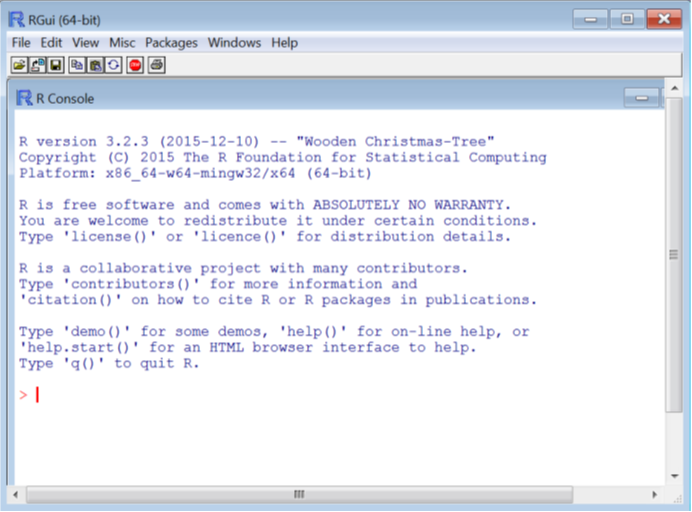
\includegraphics[width=\textwidth]{img/oef3/R-Gui-en-console}
  \end{figure}
\end{frame}

\begin{frame}
  \frametitle{R: installatie R en R Commander}
  \begin{itemize}
    \item Rcmdr:
      \begin{itemize}
        \item Gui voor R
        \item Wordt beschouwd als het beste R-alternatief tov commerciële pakketten zoals SPSS, …
        \item Ontwikkeld door Prof. John Fox
        \item Geschikt om R aan te leren aangezien bij elke analyse de onderliggende code getoond wordt
      \end{itemize}
    \item Installatie Rcmdr:
      \begin{itemize}
        \item Via Packages -- Install packages of commando install.packages(``Rcmd'', dependencies: TRUE)
        \item Vraagt de installatie van andere packages: OK
        \item Opm: gebruik ‘Single-document R interface (SDI) ipv Multiple document interface (MDI)
      \end{itemize}
    \item Installatiehulp:
      \begin{itemize}
        \item \url{http://jekyll.math.byuh.edu/other/howto/R/Rcmdr.shtml}
      \end{itemize}
  \end{itemize}
\end{frame}

\begin{frame}
  \frametitle{R: installatie R en R Commander}
  \begin{figure}[h]
    \centering
    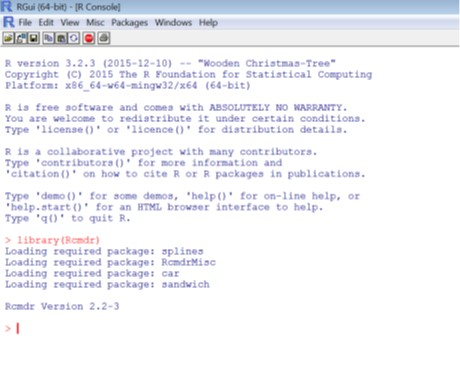
\includegraphics[width= \textwidth]{img/oef3/installatie-Rcmdr}
  \end{figure}
\end{frame}

\begin{frame}
  \frametitle{R: opstarten R Commander}
  \begin{itemize}
    \item Installatie Rcmdr:
      \begin{itemize}
        \item Start R op
        \item Daarna het commando library(Rcmdr) uitvoeren
      \end{itemize}
  \end{itemize}
\end{frame}

\begin{frame}
  \frametitle{R: opstarten R Commander}
  \begin{figure}[h]
    \centering
    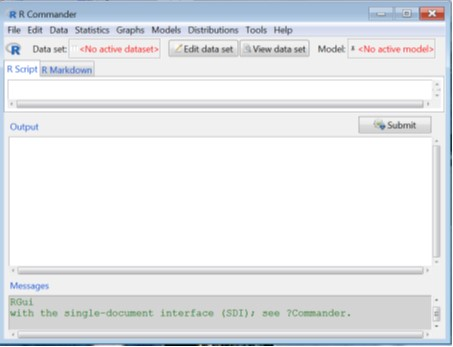
\includegraphics[width= \textwidth]{img/oef3/startscherm-R-Commander}
  \end{figure}
\end{frame}

\begin{frame}
  \frametitle{R: hulp zoeken}
  \begin{itemize}
    \item \url{https://www.youtube.com/watch?v=ZoPJGmpYJzw}
    \item ``The R Commander: A Basic-Statistics Graphical User Interface to R'' John Fox , Journal of Statistical Software 2005, Volume 14, Issue 9.
    \item \url{http://courses.statistics.com/software/RCommander/RC00.htm}
  \end{itemize}
\end{frame}

\begin{frame}
  \frametitle{Invoer data: manueel}
  \begin{itemize}
    \item Neem menu Data en kies New data set
    \item Geef een naam aan de dataset
      \begin{itemize}
        \item Geen spaties
        \item R is case sensitive
      \end{itemize}
    \item Voer de data in
    \item Geef de variabelen (kolommen) een naam door op het kolomlabel te klikken. Geef ook een datatype in.
    \item Deze dataset is nu de actieve dataset voor R Commander
  \end{itemize}
\end{frame}

\begin{frame}
  \frametitle{Invoer data: vanuit tekstbestand}
  \begin{itemize}
    \item Data -- Import data -- from tekst file
    \item Geef een naam aan de nieuwe dataset: vb. test
    \item Specifieer de kenmerken van het databestand
  \end{itemize}

  \begin{figure}[h]
    \centering
    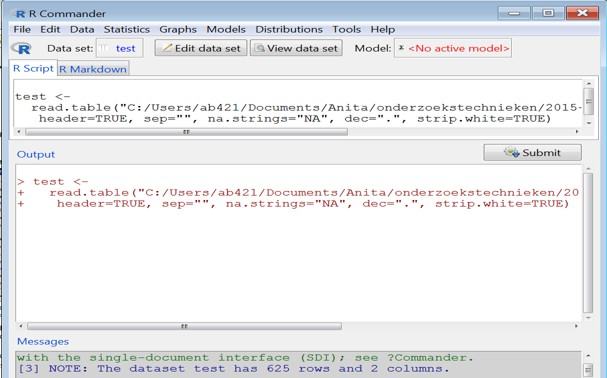
\includegraphics[width=\textwidth]{img/oef3/inlezen-tekstbestand}
  \end{figure}
\end{frame}

\begin{frame}
  \frametitle{Invoer data: vanuit Excel, SAS, SPSS, ...}
  \begin{figure}[h]
    \centering
    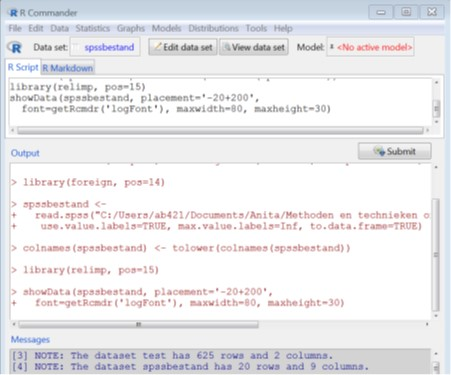
\includegraphics[width=.9\textwidth]{img/oef3/invoer-uit-spss}
  \end{figure}
\end{frame}







\section{Beschrijvende statistiek}

\begin{frame}
  \frametitle{Beschrijvende statistiek}
  \begin{itemize}
    \item Neem de dataset Studenten
    \item Bevat als variabelen:
      \begin{itemize}
        \item Id: unieke identificatie
        \item Geslacht: nominaal type
        \item Wiskunde: ordinaal type; 1 (heel slecht) … 5 (uitstekend)
        \item Leeftijd: ratiotype, discreet
        \item Lengte: ratiotype, continu
      \end{itemize}
    \item Via Statistics -- Summaries -- Active data set: overzicht van centrale maten en kwartielen per variabele
      \begin{itemize}
        \item Zijn deze allen even zinvol?
        \item Wat valt op bij de variabele ‘Geslacht’?  Waarom?
      \end{itemize}
    \item Geef de standaardafwijking, de IQR en de variatiecoëfficiënt van de variabele ‘Lengte’
      \begin{itemize}
        \item Via welk menu?
        \item Betekenis van ‘variatiecoëfficiënt'? Dimensie?
      \end{itemize}
  \end{itemize}
\end{frame}

\begin{frame}
  \frametitle{Beschrijvende statistiek: en verder \ldots}
  \begin{itemize}
    \item Beschrijvende statistiek per categorie (nominaal type):
      \begin{itemize}
        \item Bv.:
          \begin{itemize}
            \item Gemiddelde leeftijd per geslacht
            \item Gemiddelde lengte per geslacht
          \end{itemize}
        \item Statistics -- Summaries -- Table of statistics
      \end{itemize}
  \end{itemize}

\end{frame}

\begin{frame}
  \frametitle{Beschrijvende statistiek: en verder ...}

  \begin{columns}[c]

    \column{.5\textwidth}
    \begin{itemize}
      \item Aanmaken frequentietabel
        \begin{itemize}
        \item Bv.: lengte in interval ]155;165], ]165;175] en ]175;185]
        \item Via Data -- Manage variables in active data set -- Recode variables
          \begin{itemize}
            \item Geef naam aan nieuwe (categorische) variabele
            \item Geef de grenzen van de intervallen aan
          \end{itemize}
      \end{itemize}
  \end{itemize}

  \column{.5\textwidth}
  \begin{figure}
    \centering
    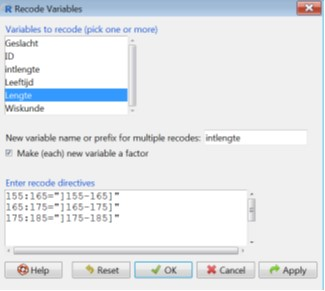
\includegraphics[width=\textwidth]{img/oef3/recode}
  \end{figure}

\end{columns}
\end{frame}

\begin{frame}
  \frametitle{Beschrijvende statistiek: en verder ...}
  \begin{columns}[c]
    \column{.5\textwidth}
    \begin{itemize}
      \item Frequentietabel via Statistics -- Summaries -- Numerical summaries
      \item Kies nu summarize by: de nieuwe variabele
    \end{itemize}

    \column{.5\textwidth}
    \begin{figure}
      \centering
      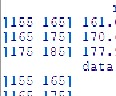
\includegraphics{img/oef3/freqtabel}
    \end{figure}
  \end{columns}
\end{frame}

\begin{frame}
  \frametitle{Grafieken}
  \begin{columns}[c]
    \column{.5\textwidth}
    \begin{itemize}
      \item Via Graphs
        \begin{itemize}
          \item Histogram van lengte
          \item Histogram van lengte per geslacht
        \end{itemize}
    \end{itemize}

    \column{.5\textwidth}
    \begin{figure}

      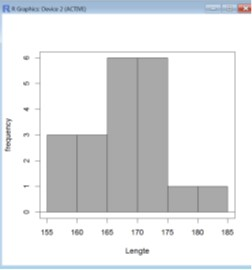
\includegraphics[width=.6\textwidth]{img/oef3/histogram-lengte}
    \end{figure}
    \begin{figure}

      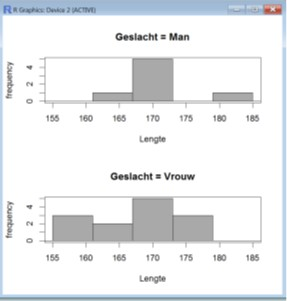
\includegraphics[width=.6\textwidth]{img/oef3/histogram-lengte-geslacht}
    \end{figure}
  \end{columns}
\end{frame}

\begin{frame}
  \frametitle{Grafieken}
  \begin{columns}[c]
    \column{.5\textwidth}
    \begin{itemize}
      \item Boxplot
        \begin{itemize}
          \item Bv.: wiskunde
          \item Bv.: leeftijd
        \end{itemize}
    \end{itemize}

    \column{.5\textwidth}
    \begin{figure}

      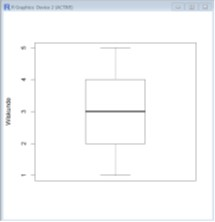
\includegraphics[width=0.6\textwidth]{img/oef3/boxplot-wiskunde}
    \end{figure}
    \begin{figure}

      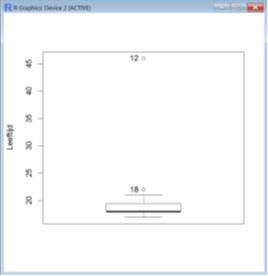
\includegraphics[width=0.6\textwidth]{img/oef3/boxplot-leeftijd}
    \end{figure}
  \end{columns}
\end{frame}

\begin{frame}
  \frametitle{Grafieken: taartdiagram}
  \begin{figure}
    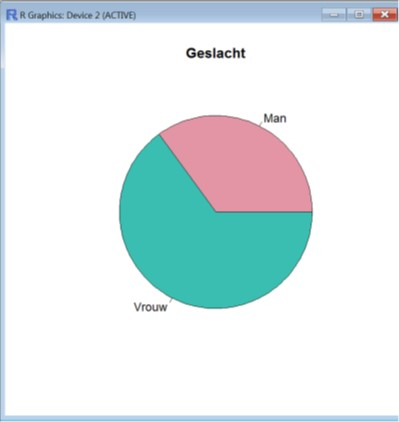
\includegraphics[width=0.5\textwidth]{img/oef3/taartdiagram-geslacht}
  \end{figure}
\end{frame}

\begin{frame}
  \frametitle{Grafieken: staafdiagram}
  \begin{figure}
    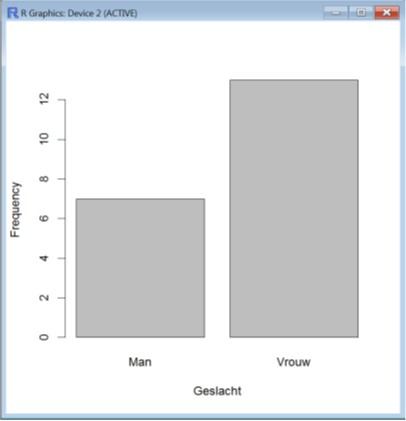
\includegraphics[width=0.5\textwidth]{img/oef3/staafdiagram-geslacht}
  \end{figure}
\end{frame}

\begin{frame}
  \frametitle{Grafieken: scatterdiagram}
  \begin{figure}
    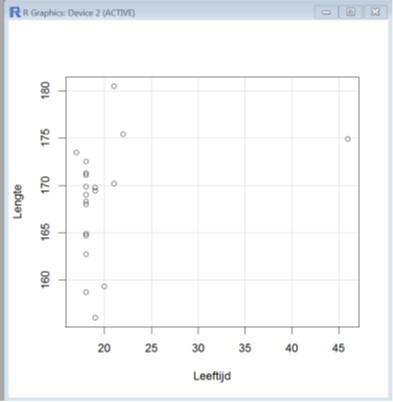
\includegraphics[width=0.5\textwidth]{img/oef3/scatterdiagram}
  \end{figure}
\end{frame}

\section{Android persistence continued}
\section{Android persistence continued}
\begin{frame}{Android persistence continued}
	Bekijk de oefeningen uit de cursus betreffende de Casus Android Persistentie. 

\end{frame}


\section{Extra oefeningen}
\subsection{Bevolking}

\begin{frame}
	\frametitle{Bevolking - opgave 1}
	Het Nationaal Instituut voor de Statistiek (NIS) beschikt over heel wat informatie o.a. ook over de bevolking. Een aangepaste versie hiervan kan je vinden in het bestand "bevolkingsgegevens aangepast.xls"
	\begin{itemize}
		\item Bereken de gemiddelden van de geboortes, sterfgevallen en echtscheidingen.
		\item Bereken de standaardafwijking van de immigratie en de emigratie.
		\item Bereken de varcoef van de Huwelijksontbindingen en van de Echtscheidingen. Conclusie?
		\item Teken een grafiek van de Bevolking t.o.v. Periode.
		\item Teken het verloop in de tijd van de Immigratie en de Emigratie.
\end{itemize}
\end{frame}

\ifoplossing
\begin{frame}[fragile]
	\lstinputlisting{Roplossingen/oef3_1var/1var-1-bevolking.R}
\end{frame}
	
\fi
\subsection{Jongeren}
\begin{frame}
	\frametitle{Jongeren - opgave 2}
	In het bestand "jongeren.xls" staat het aantal jongens en meisjes van 0 tot 18 jaar in een bepaald jaar.
		\begin{itemize}
			\item Bereken de kwartielen in de populatie van meisjes.
			\item Maak een grafiek die het aantal meisjes tegen het aantal jongens uitzet. Wat valt je op?
			\item Maak een grafiek van de verhouding tussen meisje en jongens per leeftijdscategorie.
			\item Teken de boxplot met de data van de jongens.
		\end{itemize}
\end{frame}

\ifoplossing
	\begin{frame}
		\lstinputlisting{Roplossingen/oef3_1var/1var-2-jongeren.R}
	\end{frame}

\fi
\subsection{Lengte \& Gewicht}
\begin{frame}
	\frametitle{Lengte en gewicht - opgave 3}
	In het bestand "lengtegewicht.txt" zien we de resultaten van de metingen in een klas.
		\begin{itemize}
			\item Bepaal de gemiddelde lengte en het gemiddeld gewicht.
			\item Bereken de variatiecoëfficiënt van beide variabelen.  Conclusie?
			\item Maak voor de variabele lengte intervallen aan van 5 cm en genereer de frequentietabel.
			\item Zet deze frequenties uit in een histogram.
		\end{itemize}
\end{frame}

\ifoplossing
\begin{frame}[fragile]
	\lstinputlisting{Roplossingen/oef3_1var/1var-3-lengtegewicht.R}
\end{frame}
\fi

\end{document}
